```latex
\documentclass[12pt,a4paper]{article}

% ---------------- Packages ----------------
\usepackage{geometry}
\geometry{margin=1in}

\usepackage{booktabs}
\usepackage{tabularx}
\usepackage{titlesec}
\usepackage{listings}
\usepackage{xcolor}
\usepackage{graphicx}
\usepackage{setspace}
\usepackage{hyperref}
\usepackage{tocloft}
\usepackage{longtable}
\usepackage{float}
\usepackage{caption}

% ---------------- Section Formatting ----------------
\titleformat{\section}{\Large\bfseries}{\thesection}{1em}{}
\titleformat{\subsection}{\large\bfseries}{\thesubsection}{1em}{}

% ---------------- Code Listing Setup ----------------
\lstset{
    language=C++,
    basicstyle=\ttfamily\small,
    keywordstyle=\color{blue}\bfseries,
    stringstyle=\color{red},
    commentstyle=\color{green!60!black},
    numbers=left,
    numberstyle=\tiny\color{gray},
    stepnumber=1,
    frame=single,
    breaklines=true,
    showspaces=false,
    showstringspaces=false,
    showtabs=false
}

\begin{document}

% ---------------- Title Page ----------------
\begin{titlepage}
\centering
\vspace*{2cm}

{\Huge \textbf{UML Diagrams Document}}\\[0.5cm]
{\Large \textbf{NexusNotes}}\\[0.5cm]
{\large Centralized Academic Resource Platform}\\[2cm]

\textbf{Project Team: Code Club}\\[0.5cm]

Ramasani Adi Pranav -- 24CSB0A57\\
Syed Mohammad Sami -- 24CSB0A77\\
Janapala Harsha Vardhan Reddy -- 24CSB0A28\\[2cm]

\vfill

{\large \textbf{Version 1.0}}\\
{\large \today}

\end{titlepage}

\tableofcontents
\newpage

% ---------------- Introduction ----------------
\section{Introduction}

This document provides a comprehensive overview of the Unified Modeling Language (UML) diagrams for the Nexus Notes platform. Nexus Notes is a centralized academic knowledge platform that integrates students, faculty, and academic resources into a unified digital ecosystem. The following sections describe the Use Case, Sequence, Collaboration, and Activity diagrams that represent the system's architecture and interactions.

% ---------------- Use Case Diagram ----------------
\section{Use Case Diagram}

The Use Case Diagram provides a high-level representation of the interactions between system actors and the core functionalities of the Nexus Notes platform.

\begin{figure}[H]
\centering
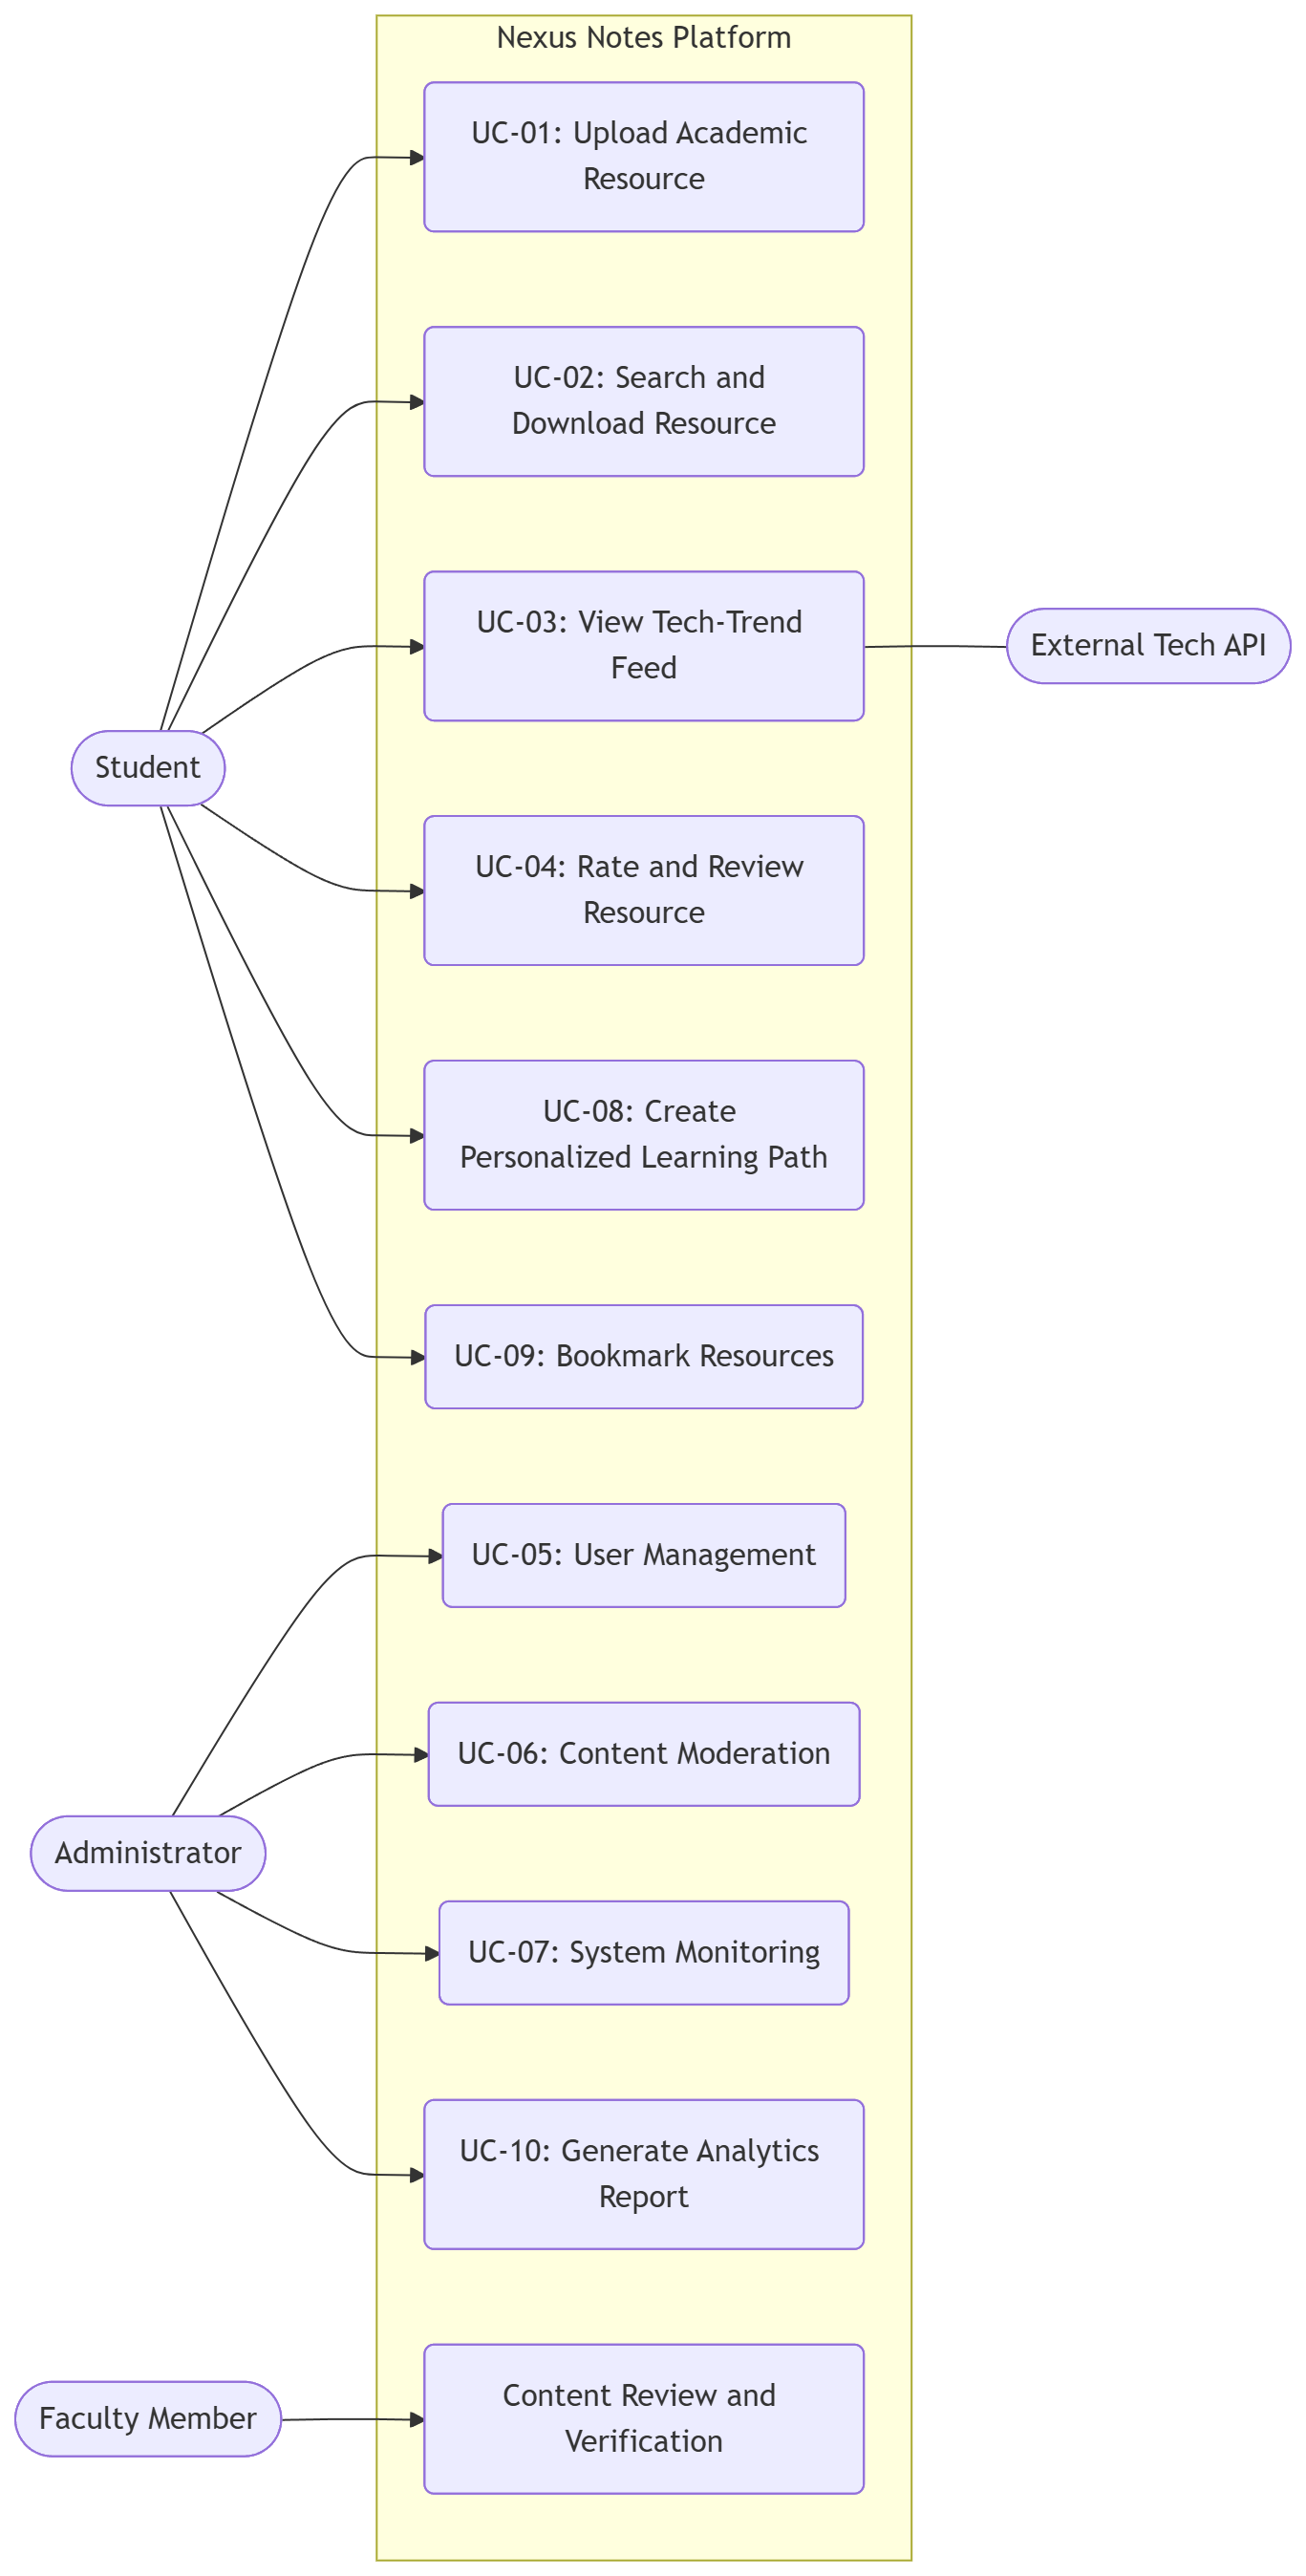
\includegraphics[width=0.8\textwidth]{mermaid-diagram-2026-03-14-094337.png}
\caption{Use Case Diagram for Nexus Notes Platform}
\end{figure}

\subsection{Explanation}

The main actors involved in the system are Student, Administrator, Faculty Member, and External Tech API.

\begin{itemize}

\item \textbf{Student:} Uploads academic resources, searches and downloads study materials, views technology updates, and rates resources.

\item \textbf{Administrator:} Manages users, moderates uploaded content, and monitors the system performance.

\item \textbf{Faculty Member:} Reviews and verifies academic content uploaded to the platform.

\item \textbf{External Tech API:} Provides real-time technological updates for the Tech-Trend Feed feature.

\end{itemize}

% ---------------- Sequence Diagram ----------------
\section{Sequence Diagram: Upload Academic Resource (UC-01)}

The Sequence Diagram illustrates the step-by-step interaction that occurs when a student uploads an academic resource.

\begin{figure}[H]
\centering
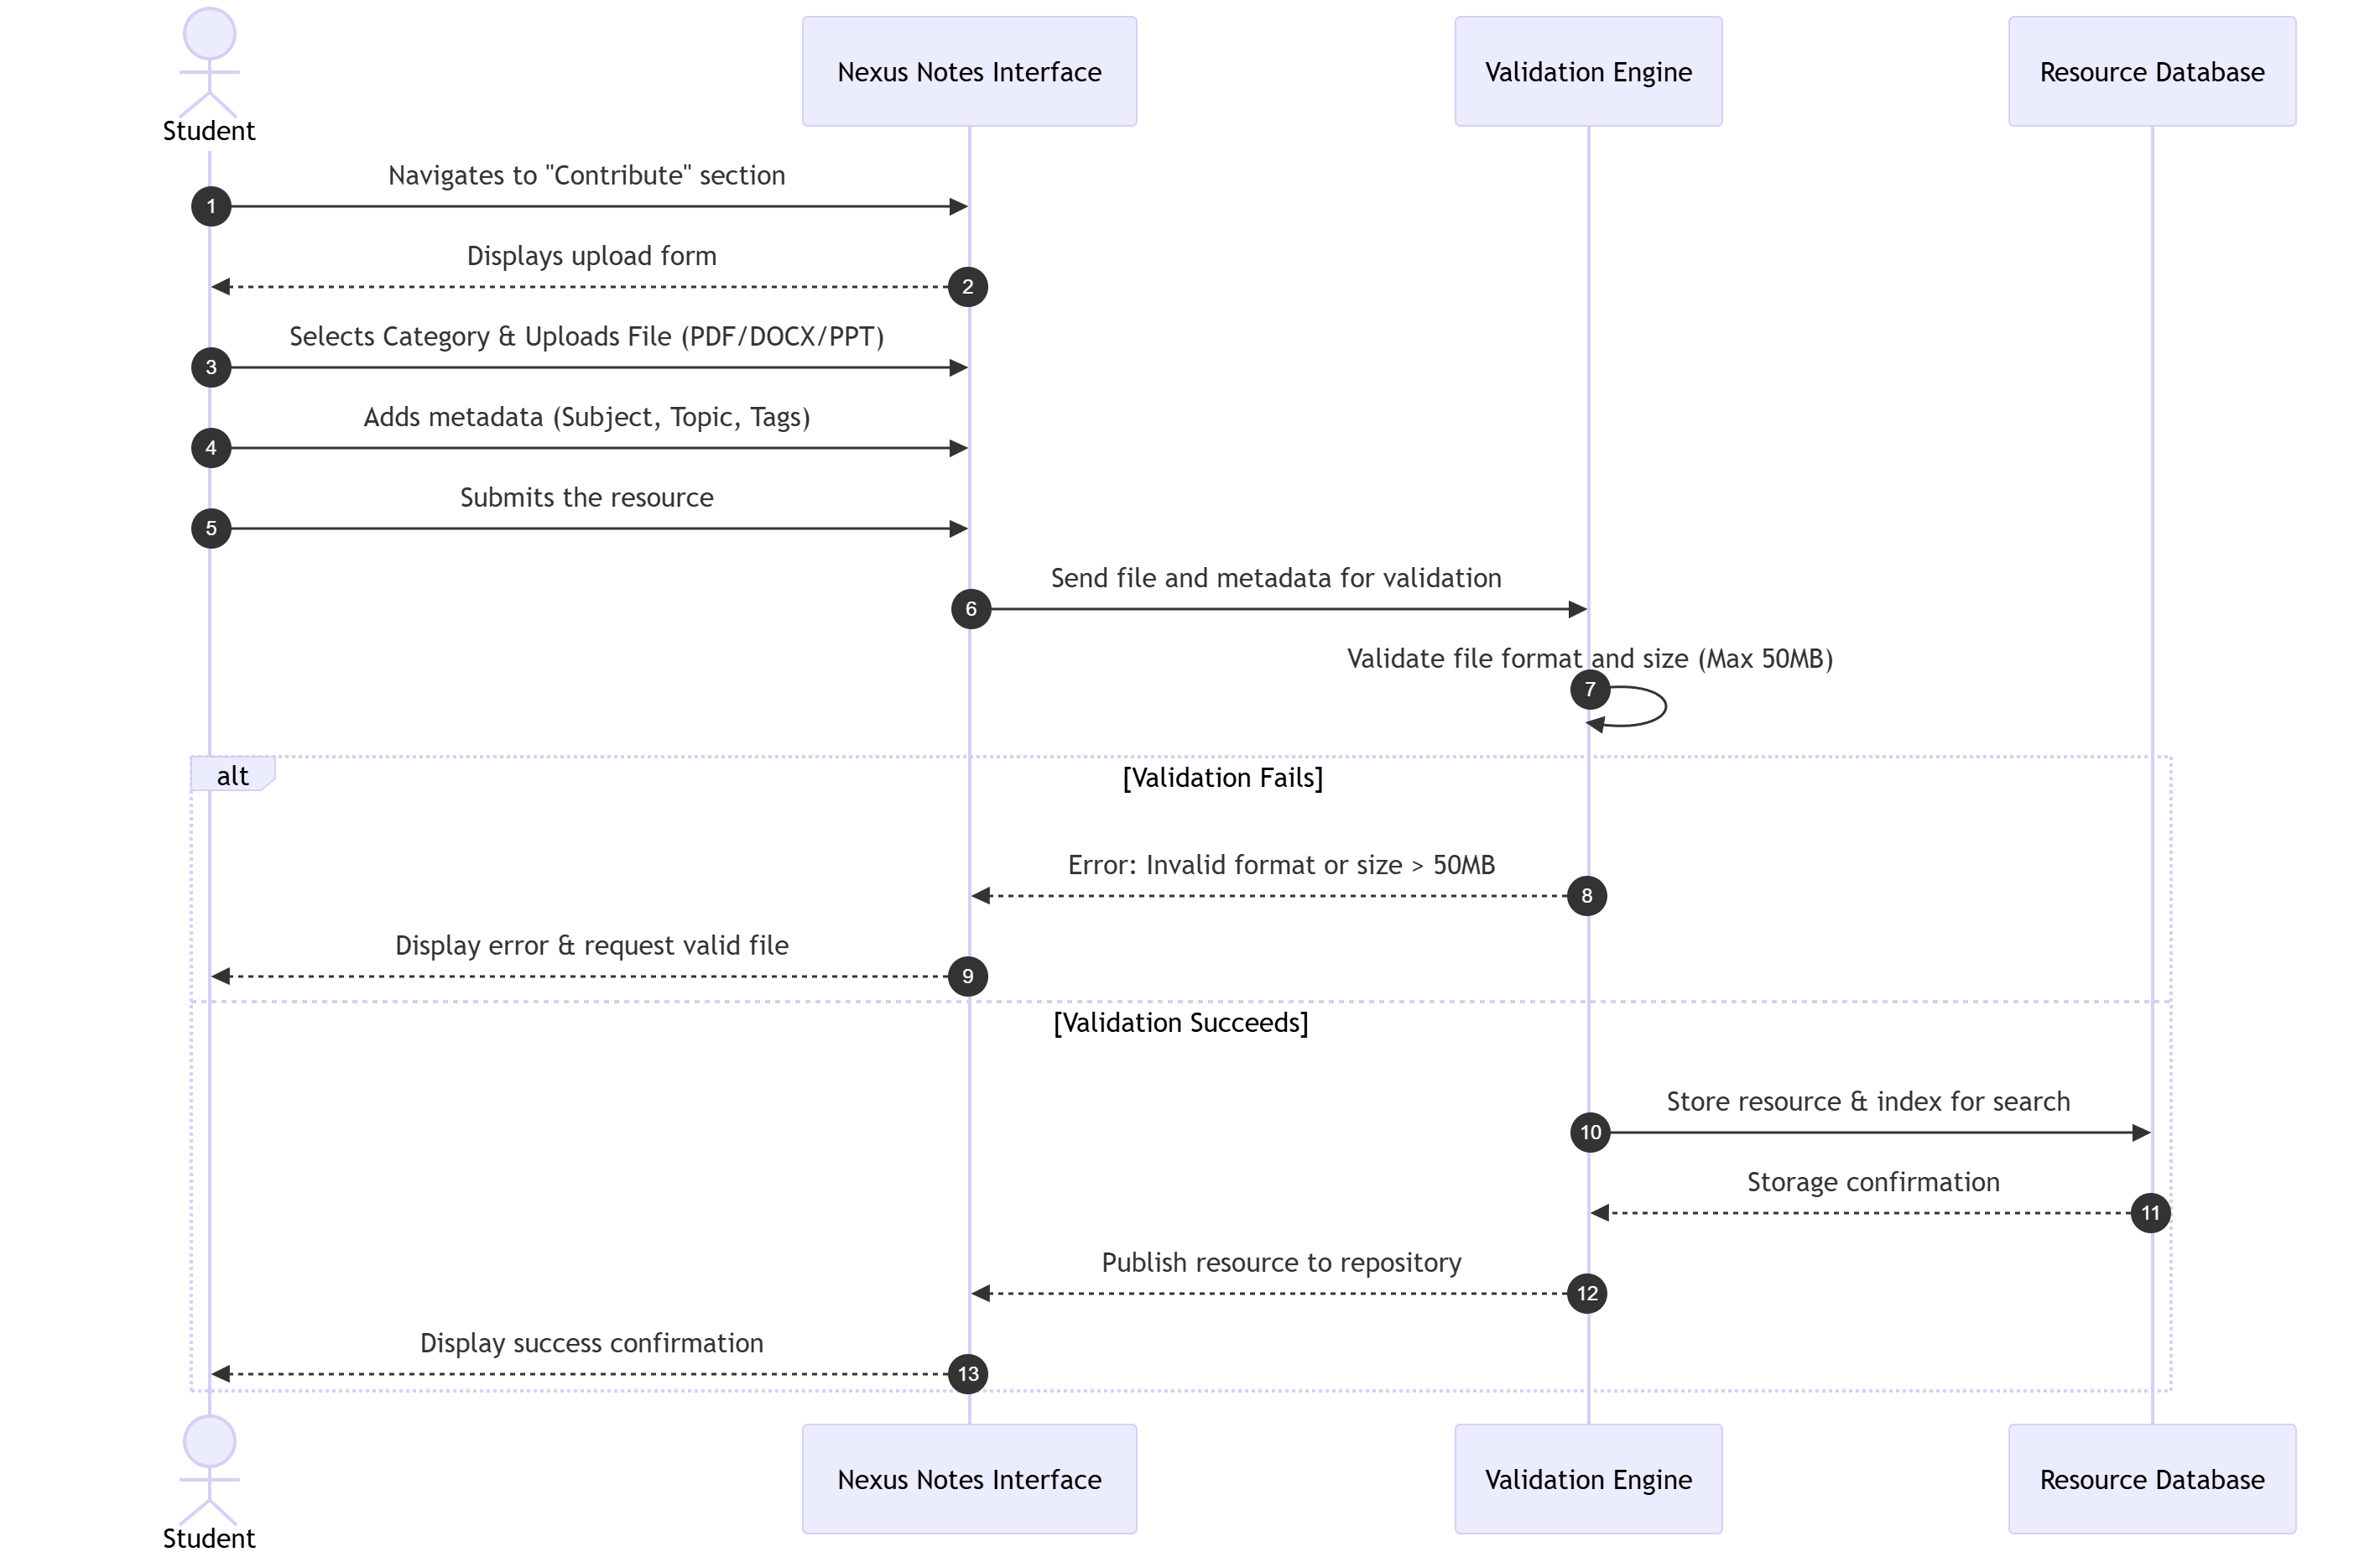
\includegraphics[width=\textwidth]{mermaid-diagram-2026-03-14-094407.png}
\caption{Sequence Diagram for UC-01: Upload Academic Resource}
\end{figure}

\subsection{Explanation}

\begin{itemize}

\item The student navigates to the Contribute section where the upload interface is displayed.

\item The student selects the category, uploads the file (PDF, DOCX, PPT), adds metadata, and submits the resource.

\item The system validates the uploaded file format and ensures that the file size is within the allowed limit.

\item If validation fails, the system displays an error message requesting the correct file format.

\item If validation succeeds, the resource is stored in the database and indexed for search, and a confirmation message is displayed.

\end{itemize}

% ---------------- Collaboration Diagram ----------------
\section{Collaboration Diagram: Search and Download Resource (UC-02)}

The Collaboration Diagram shows how different system components communicate with each other during the process of searching and downloading academic resources.

\begin{figure}[H]
\centering
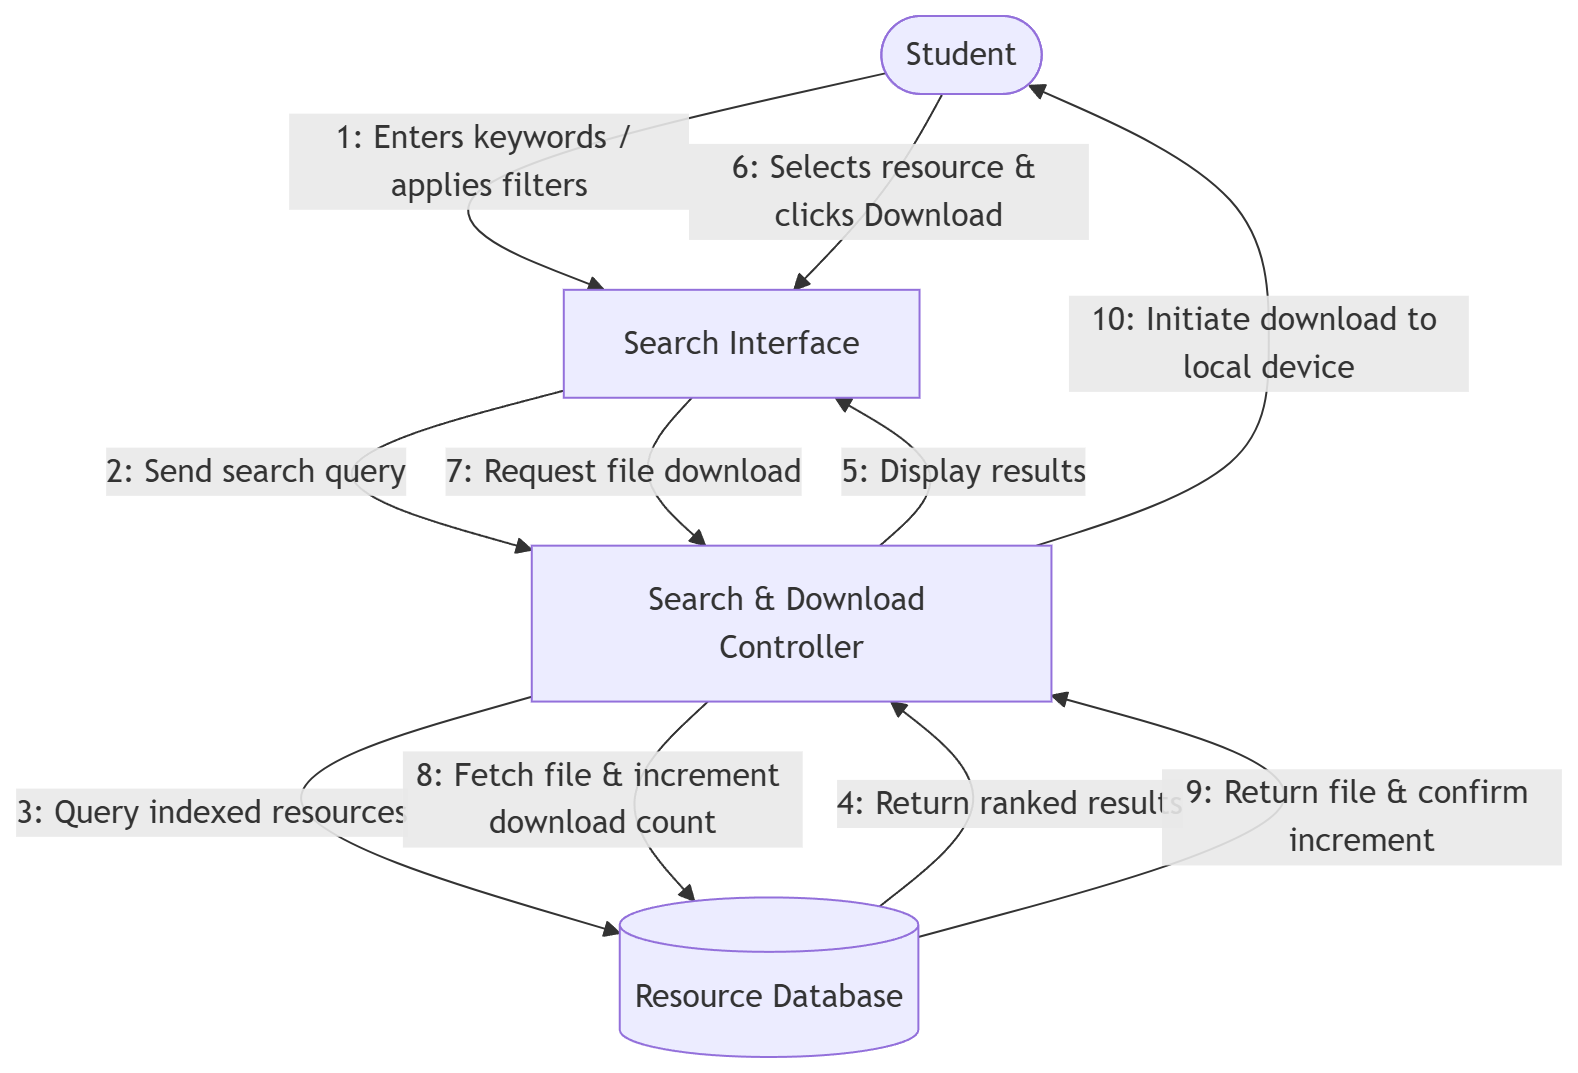
\includegraphics[width=0.9\textwidth]{mermaid-diagram-2026-03-14-094605.png}
\caption{Collaboration Diagram for UC-02: Search and Download Resource}
\end{figure}

\subsection{Explanation}

\begin{itemize}

\item The student enters keywords or filters through the search interface.

\item The request is sent to the controller which queries the resource database.

\item The database returns the results ranked based on relevance and ratings.

\item The results are displayed to the student.

\item When the student selects a resource and clicks download, the system retrieves the file, updates the download count, and initiates the download.

\end{itemize}

% ---------------- Activity Diagram ----------------
\section{Activity Diagram: Content Moderation (UC-06)}

The Activity Diagram represents the workflow followed by administrators during content moderation.

\begin{figure}[H]
\centering
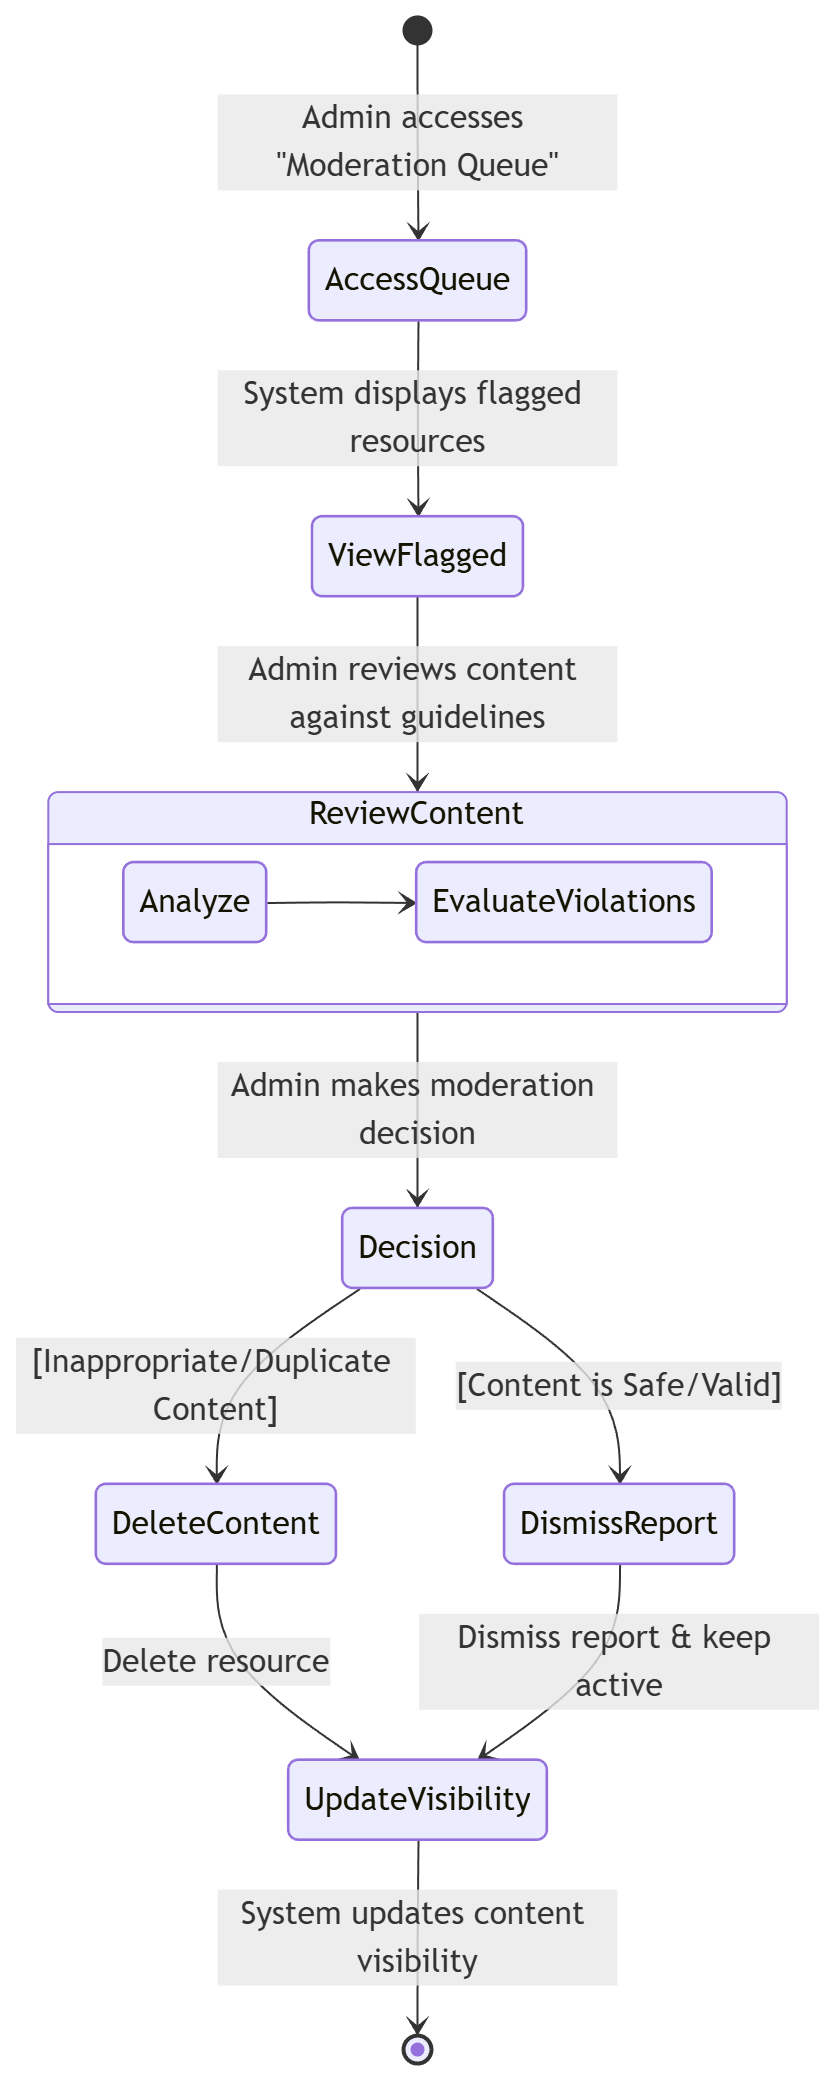
\includegraphics[width=0.6\textwidth]{mermaid-diagram-2026-03-14-094618.png}
\caption{Activity Diagram for UC-06: Content Moderation}
\end{figure}

\subsection{Explanation}

\begin{itemize}

\item The administrator opens the moderation queue where flagged resources are displayed.

\item The administrator reviews the content against platform guidelines.

\item If the content violates rules or is duplicated, the administrator deletes the resource.

\item If the report is invalid, the administrator dismisses the report.

\item The system updates the content visibility status based on the administrator's decision.

\end{itemize}

\end{document}
```
